\documentclass[paper=letter, fontsize=12pt]{article}
\usepackage{geometry}
\geometry{margin=1in}
\usepackage{graphicx}
\graphicspath{{images/}}
\usepackage{amssymb}
\usepackage{enumitem}
\usepackage{amsmath}
\usepackage{mathrsfs}
\usepackage{algorithm2e}

%opening
\title{Compsci 571 HW6}
\author{Yilin Gao (yg95)}

\begin{document}

\maketitle
\section{Neural Networks and Universal Approximation Theorem}

\subsection{}

\begin{enumerate}[label=(\alph*)]
	\item The NN architecture is like following:
			
	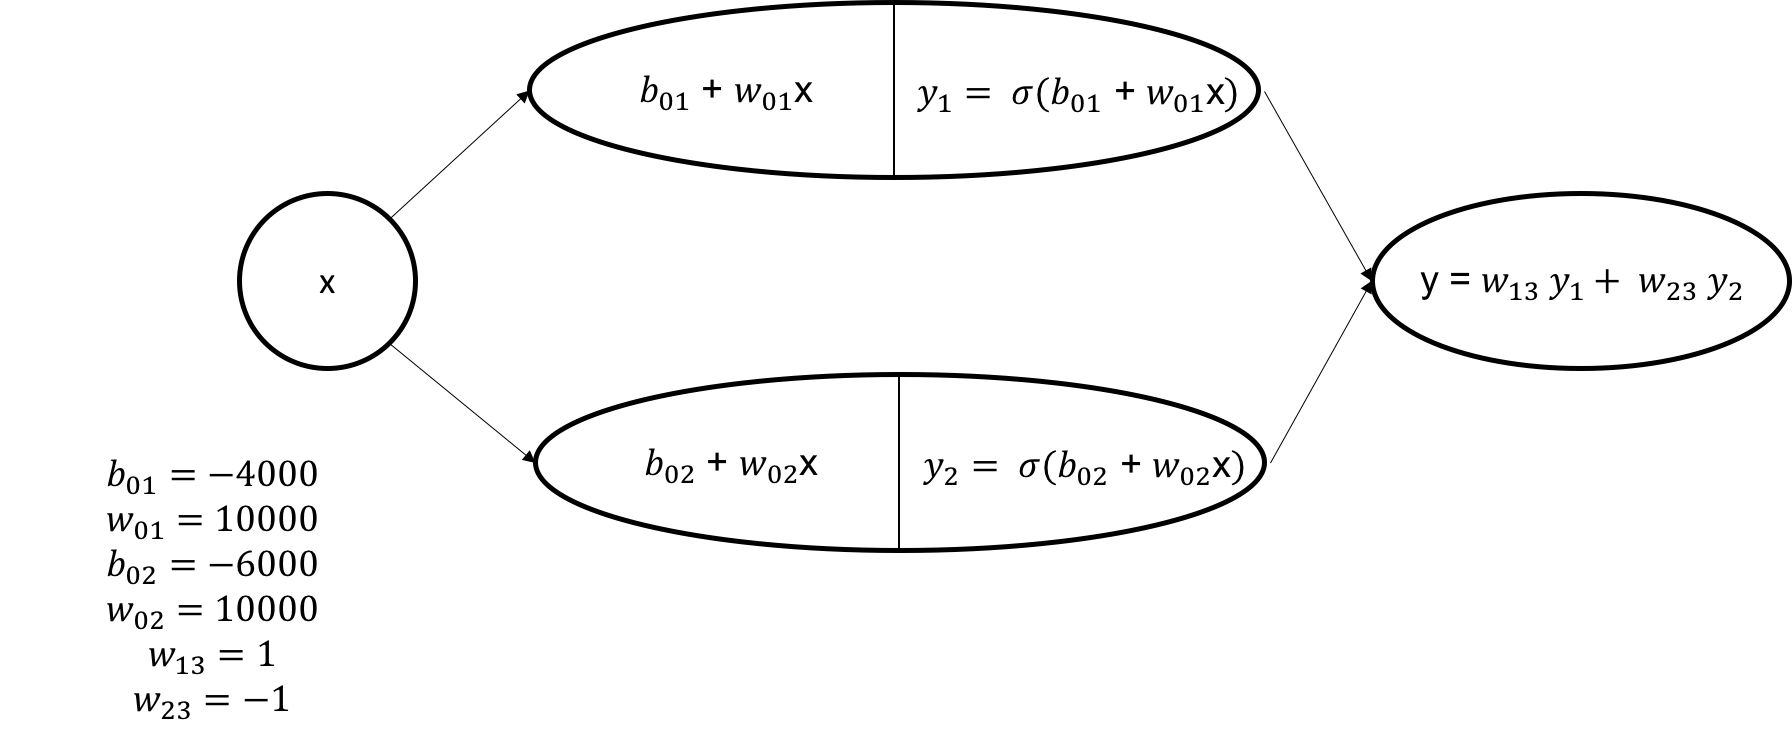
\includegraphics[scale=0.4]{q1a.png}
			 
	The implementation is in \verb|q1.ipynb|. The approximated function is as following:
	
	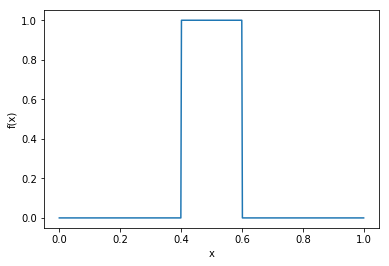
\includegraphics[scale=0.6]{q1a2.png}
			 
	The minimal number of hidden neurons is 2, because the bump is a combination of 2 step functions, and each neuron (with the sigmoid activation function) is able to approximate one step function with any given step direction, location and height.
	
	\item In the NN, $w_{01}$ determines the steepness of the step-up part of the bump, $w_{02}$ determines the steepness of the step-down part of the bump. $-\frac{b_{01}}{w_{01}}$ determines the step-up location, $-\frac{b_{02}}{w_{02}}$ determines the step-down location. And $w_{13}$ and $w_{23}$ determine the height of the bump.
\end{enumerate}

\subsection{}

\begin{enumerate}[label=(\alph*)]
	\item The NN architecture is like following:
	
	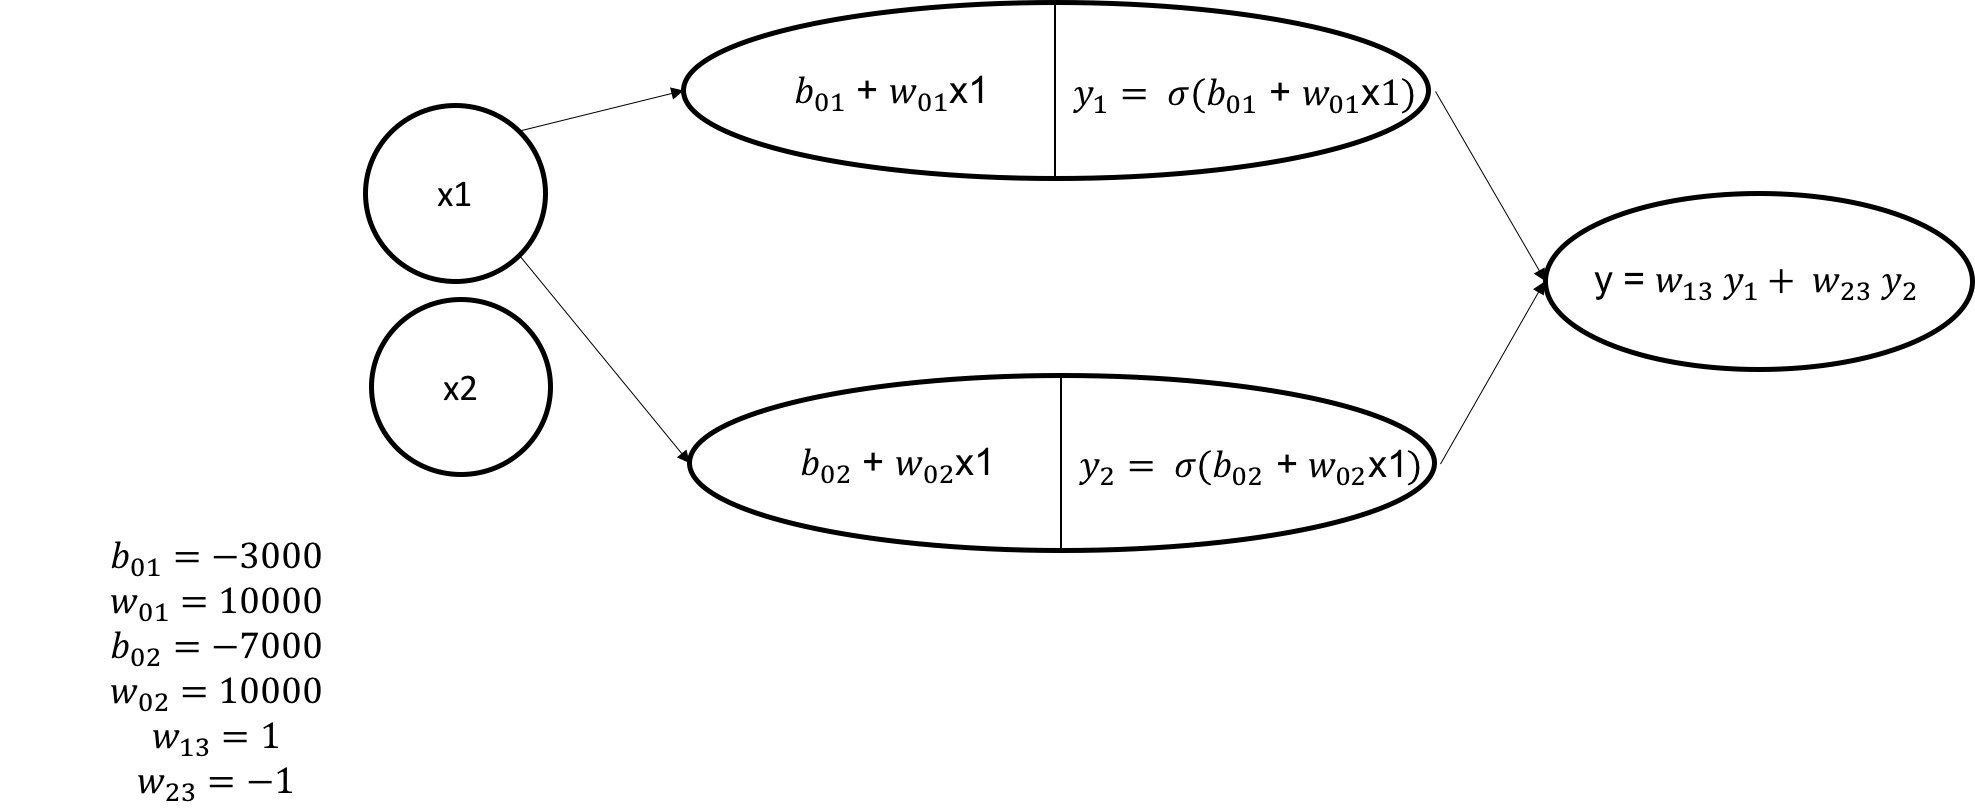
\includegraphics[scale=0.4]{q12a1.png}
	
	There is no edge between the input cell for $x_2$ and the hidden layer.
	
	The implementation is in \verb|q1.ipynb|. The approximated function is as following:
	
	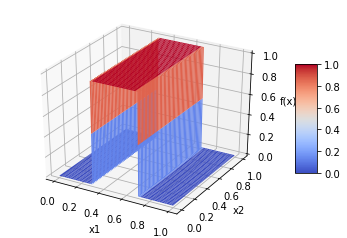
\includegraphics[scale=0.6]{q12a2.png}
	
	The minimal number of hidden neurons is 2.  Because the 2D bump is only in the direction of $x_1$, so we can regard it same as the one in part 1, and ignore the input $x_2$.
	
	\item The NN architecture is like following:
	
	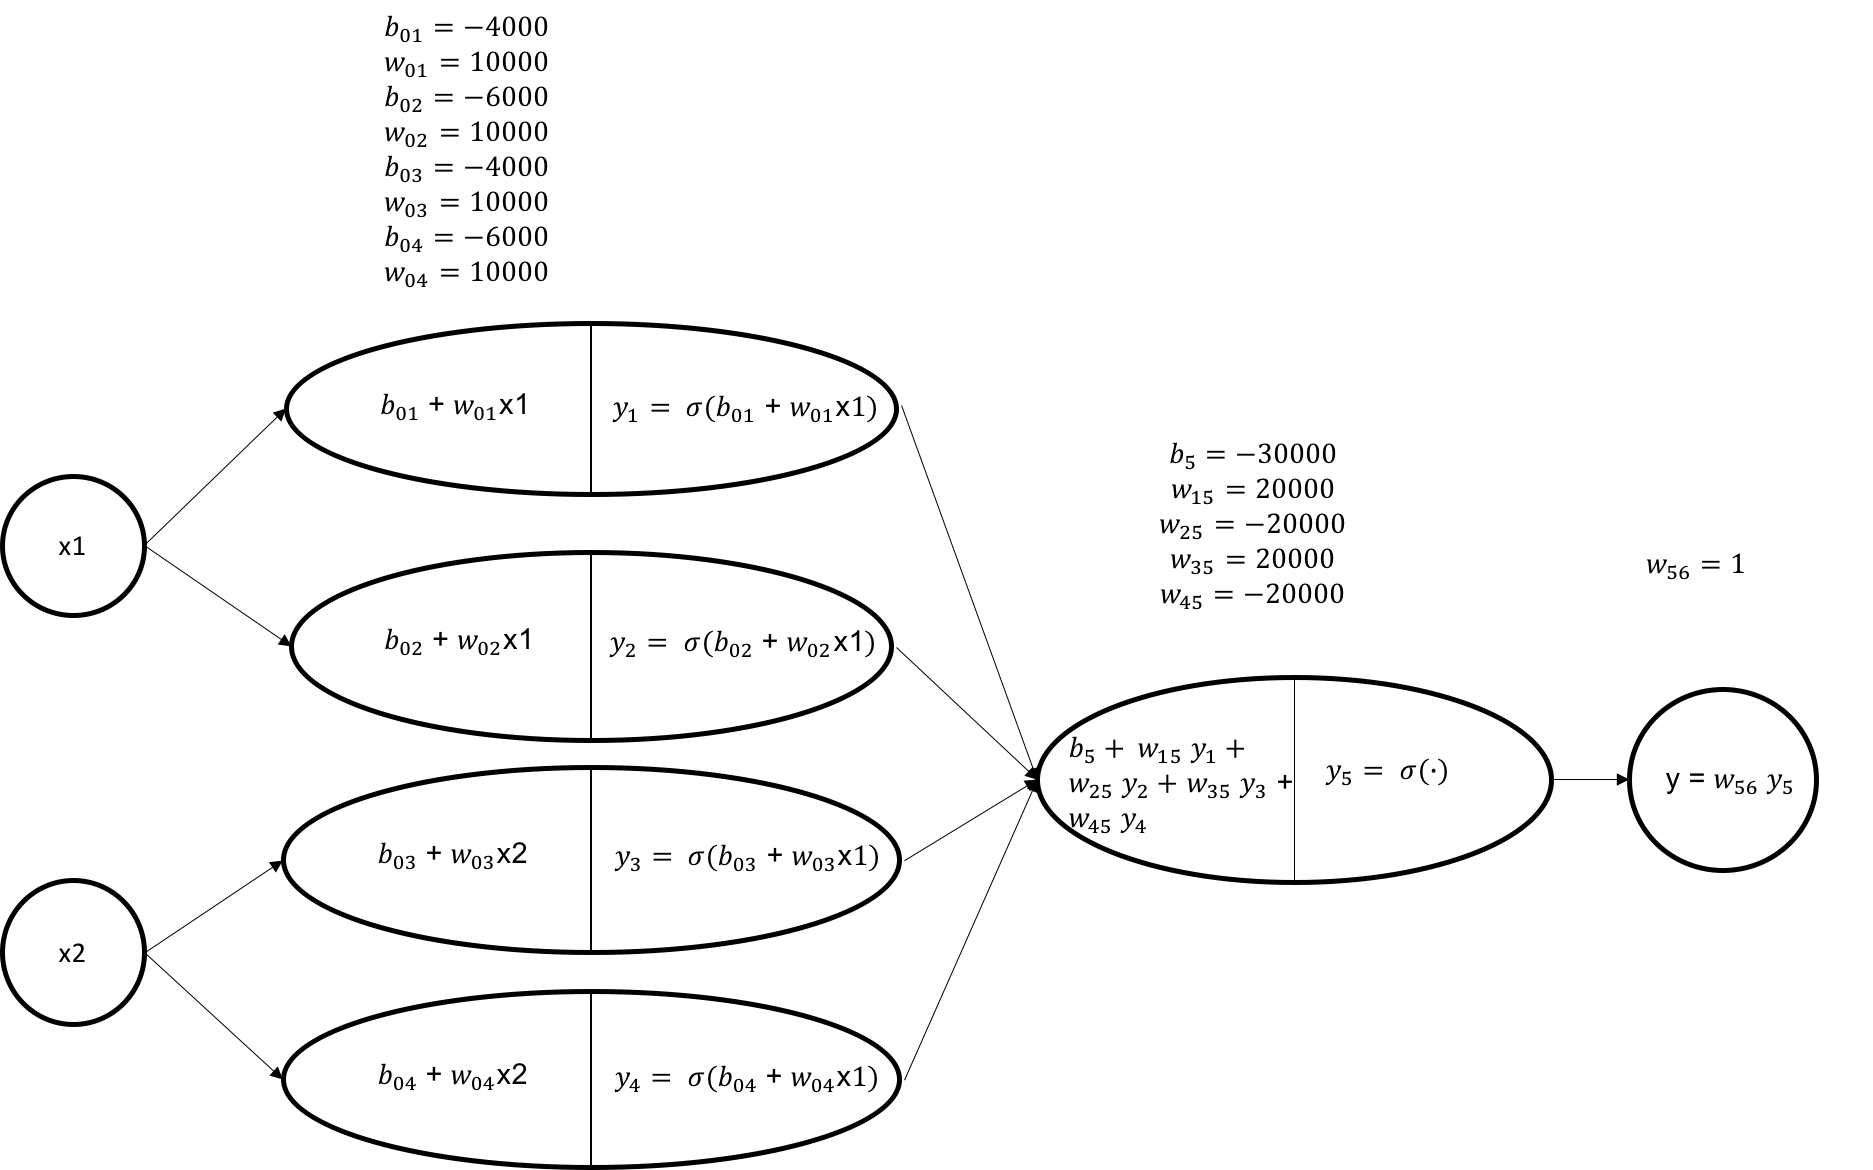
\includegraphics[scale=0.4]{q12b1.png}
	
	The implementation is in \verb|q1.ipynb|. The approximated function is as following:
	
	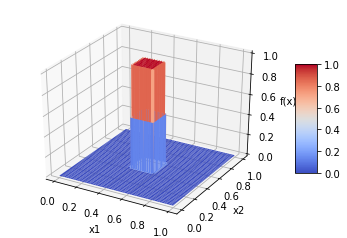
\includegraphics[scale=0.6]{q12b2.png}
	
	The minimal number of hidden neuron in the first layer is 4. Because the 2D bump is a combination of a bump in $x_1$ direction and another bump in $x_2$ direction, and each bump needs 2 hidden neurons according to previous question.
	
	\item For a grid $(x_1, x_2)$ such that $x_1 \in [x_1^*, x_1^* + \frac{1}{n}]$ and $x_2 \in [x_2^*, x_2^* + \frac{1}{n}]$, assume the tower function we use to approximate has height $h^* = f(x_1^*, x_2^*)$.
	
	Because the grid is small enough, we can assume for any fixed $x_2^0$, $f(x_1, x_2^0)$ is linear with $x_1 \in [x_1^*, x_1^* + \frac{1}{n}]$, and for any fixed $x_1^0$, $f(x_1^0, x_2)$ is linear with $x_2 \in [x_2^*, x_2^* + \frac{1}{n}]$. So we have: $f(x_1, x_2^0) = \frac{\partial f(x_1, x_2^0)}{\partial x_1} (x_1 - x_1^*)$ for $x_1 \in [x_1^*, x_1^* + \frac{1}{n}]$, and $f(x_1^0, x_2) = \frac{\partial f(x_1^0, x_2)}{\partial x_2} (x_2 - x_2^*)$ for $x_2 \in [x_2^*, x_2^* + \frac{1}{n}]$. 
	
	Because the maximum absolute value of the gradient for both directions is $t$, $|\frac{\partial f(x_1, x_2^0)}{\partial x_1}| \leq t$, and $|\frac{\partial f(x_1^0, x_2)}{\partial x_2}| \leq t$.
	
	The approximation error on the grid = $\int_{x_1^*}^{x_1^*+\frac{1}{n}} \int_{x_2^*}^{x_2^*+\frac{1}{n}} [f(x_1, x_2) - h^*] dx_1 dx_2$. If we view it geometrically, we can easily find under this setting, it is a regular 3D object that we can calculate its volume with know data (like following). When $|\frac{\partial f(x_1, x_2^0)}{\partial x_1}| = t$, and $|\frac{\partial f(x_1^0, x_2)}{\partial x_2}| = t$, its maximal volume is $\frac{t}{n^3}$.
	
	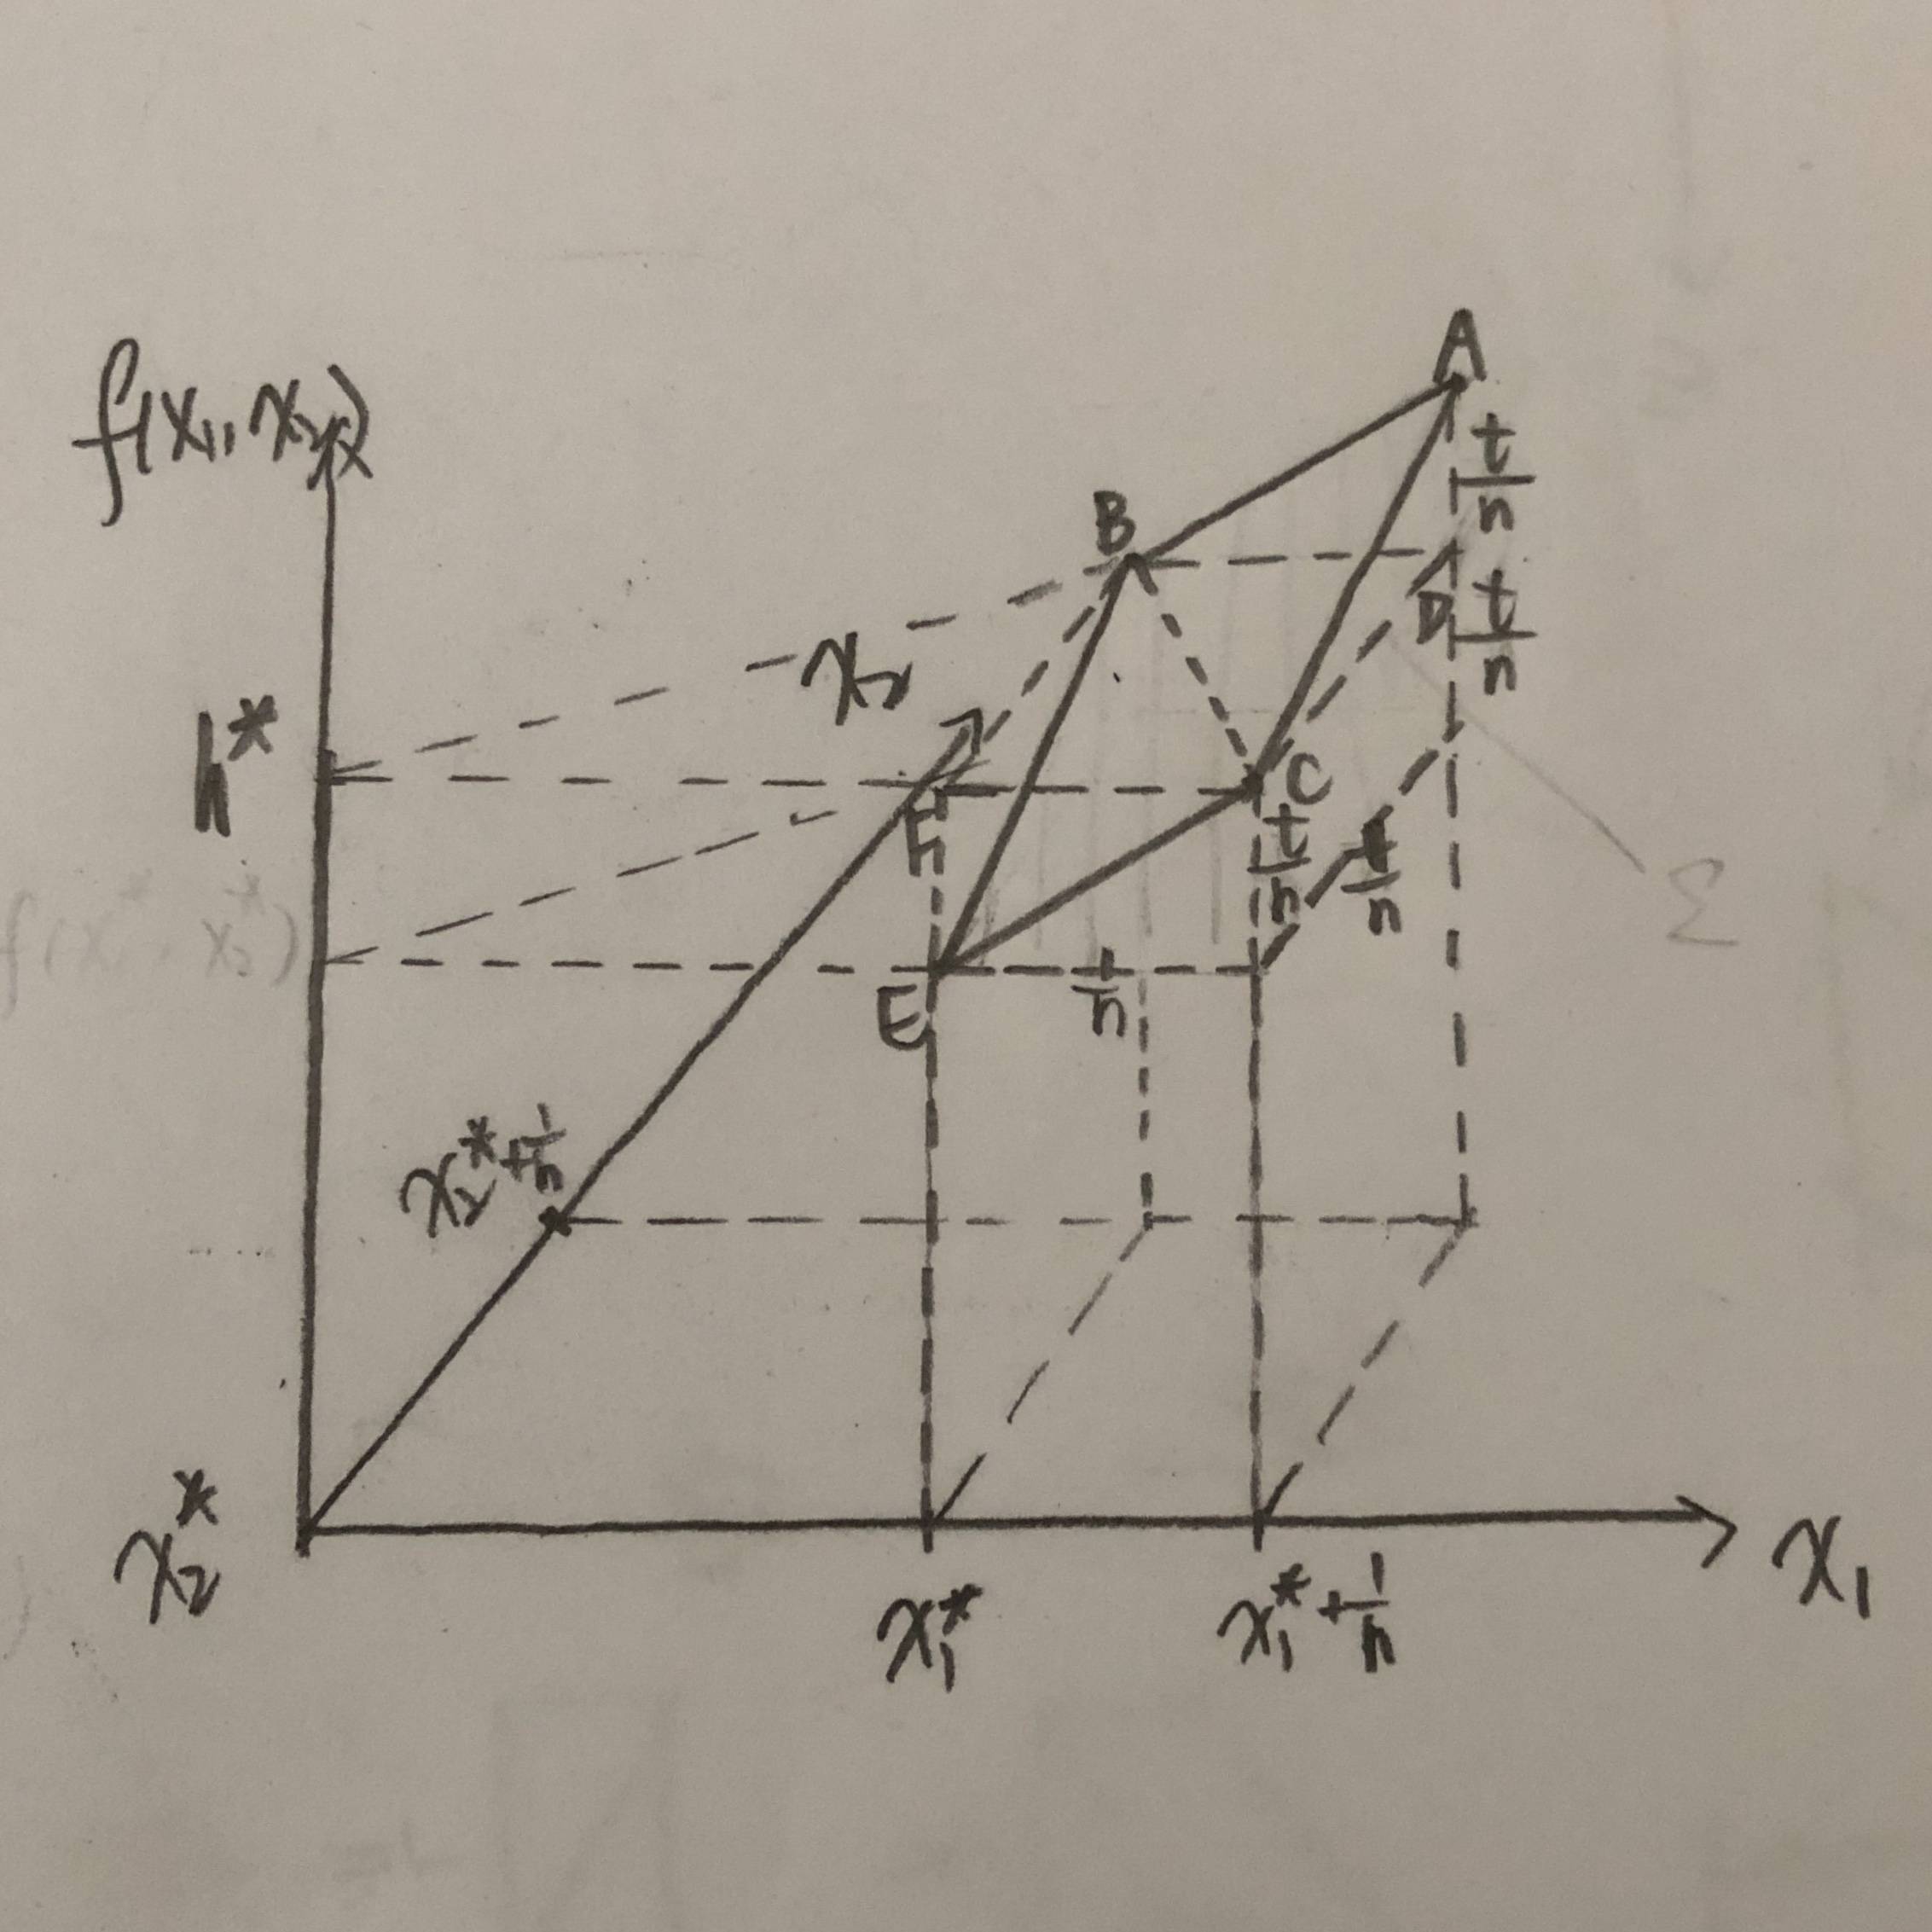
\includegraphics[scale=0.3]{q12c.png}
	
	So we have $\frac{t}{n^3} \leq \epsilon$, $n \geq \sqrt[3]{\frac{t}{\epsilon}}$. So the minimum number of tower functions to make such approximation is $n^2 = \sqrt[3]{\frac{t^2}{\epsilon^2}}$.
	
	One tower function has 5 hidden neurons in total. So the total number of required hidden neurons = $5 \sqrt[3]{\frac{t^2}{\epsilon^2}}$. When the gradient limit is larger, the total required number of hidden neurons is also larger. When the error bound is larger, the total required number of hidden neurons is smaller.
	
\end{enumerate}

\section{EM}
\begin{enumerate}[label=(\alph*)]
	\item Notations used:
	
	$i$: index for laundry visit, $i \in \{1, \dots, m\}$,
	
	$z_i$: the machine used in visit $i$, $z_i \in \{1, 2\}$,
	
	$X_i$: random variable to represent possible number of failed cycles of the chosen machine in visit $i$, $X_i \in [0, n]$,
	
	$x_i$: the observed number of failed cycles of the chosen machine in visit $i$, $x_i \in [0, n]$,
	
	$w_{ik}$: the probability to use machine $k$ in the laundry visit $i$, $k \in \{1, 2\}$, and $\sum_{k = 1}^{2} w_{ik} = 1$ for $\forall i$,
	
	$\theta_k$: the probability that machine $k$ breaks down, $k \in \{1, 2\}$.
	
	So we could have: $P(z_i = k | \vec{w}) = w_{ik}$.
	
	And we could see that given $z_i = k$ and $\theta_{k}$, $X_i$ follows Binomial distribution $(n, \theta_{k})$, $P(X_i = x_i | z_i = k, \theta_k) = \binom{n}{x_i} \theta_k^{x_{i}} (1-\theta_k)^{(n-x_{i})}$.
	
	The EM algorithm works as following:
	
	\begin{algorithm}[H]
		Initialize $\vec{w}$ and $\vec{\theta}$ as $\vec{w}^0$ and $\vec{\theta}^0$\;
		\For{$t = 0, 1, \dots $ }{
			E step: Compute $P(z_i = k | x_i, \vec{w}_t, \vec{\theta}_t) =: \gamma_{ik}^{t+1}$ \;
			M step: Maximize the auxilary function $A(\vec{w}, \vec{\theta}, \vec{w}_t, \vec{\theta}_t)$ by choosing $\vec{w}^{t+1}$ and $\vec{\theta}^{t+1}$.
			
			\If{$\vec{w}$ and $\vec{\theta}$ have converged}{Break the for loop\;}
		}
	\end{algorithm}
	
	So in $t$'th E step:
	
	$\gamma_{ik}^{t+1} =: P(z_i = k | x_i, \vec{w}^t, \vec{\theta}^t) = \frac{P(z_i = k, X_i = x_i | \vec{w}^t, \vec{\theta}^t)}{P(X_i = x_i | \vec{w}^t, \vec{\theta}^t)} = \frac{P(X_i = x_i | z_i = k, \vec{w}^t, \vec{\theta}^t) P(z_i = k | \vec{w}^t, \vec{\theta}^t)}{P(X_i = x_i | \vec{w}^t, \vec{\theta}^t)} = \frac{\binom{n}{x_i} {(\theta_k^t)}^{x_{i}} {(1-\theta_k^t)}^{(n-x_{i})} w_{ik}^t}{\sum_{k = 1}^{2}(\binom{n}{x_i} {(\theta_k^t)}^{x_{i}} {(1-\theta_k^t)}^{(n-x_{i})} w_{ik}^t) } = \frac{ {(\theta_k^t)}^{x_{i}} {(1-\theta_k^t)}^{(n-x_{i})} w_{ik}^t}{\sum_{k = 1}^{2}( {(\theta_k^t)}^{x_{i}} {(1-\theta_k^t)}^{(n-x_{i})} w_{ik}^t) }$.
	
	In $t$'th M step:
	
	$A(\vec{w}, \vec{\theta}, \vec{w}_t, \vec{\theta}_t) = \sum_{i = 1}^{m} \sum_{k = 1}^{2} \gamma_{ik}^{t+1} \log P(X_i = x_i, z_i = k | \vec{w}, \vec{\theta}) = \sum_{i = 1}^{m} \sum_{k = 1}^{2} \gamma_{ik}^{t+1} \log P(z_i = k | \vec{w}, \vec{\theta}) P(X_i = x_i | z_i = k, \vec{w}, \vec{\theta}) = \sum_{i = 1}^{m} \sum_{k = 1}^{2} \gamma_{ik}^{t+1} \log [w_{ik} \binom{n}{x_i} \theta_k^{x_{i}} (1-\theta_k)^{(n-x_{i})}] = \sum_{i = 1}^{m} \sum_{k = 1}^{2} \gamma_{ik}^{t+1} [\log w_{ik} + \log \binom{n}{x_i} + x_i \log \theta_{k} + (n-x_i) \log (n - \theta_{k})]$
	
	We need to maximize $A(\vec{w}, \vec{\theta}, \vec{w}_t, \vec{\theta}_t)$ subject to the constraint that $\sum_{k = 1}^{2} w_{ik} = 1$ for $\forall i$.
	
	With the Lagrangian method, set the partial derivatives of $A(.)$ w.r.t. $\theta_{k}$ and $w_{ik}$ equal to 0, we could get $\theta_{k}^{t+1} = \frac{\sum_{i = 1}^{m} \gamma_{ik}^{t+1} x_i}{n \sum_{i = 1}^{m} \gamma_{ik}^{t+1}}$, and $w_{ik}^{t+1} = \frac{\gamma_{ik}^{t+1}}{\sum_{k = 1}^{2} \gamma_{ik}^{t+1}}$, for $k = \{1, 2\}$ and $i \in [1, m]$.
	
	\item See the implementation in \verb|q2.ipynb|. For the specific simulated data left in the notebook, and the initial parameter $w_{ik}^0 =  0.5$ $\forall i \forall k$ and $\vec{\theta}^0 = [0.9, 0.1]$, the estimated $\hat{\theta}_1 = 0.7725$ and estimated $\hat{\theta}_2 = 0.305$. The estimation changes as the simulated data and initialization change.
\end{enumerate}

\section{Clustering}
\begin{enumerate}[label=(\alph*)]
	\item See the implementation in \verb|q3.ipynb|.
	
	\item See the implementation in \verb|q3.ipynb|.
	
	\item The empirical clustering results on the dataset with both algorithms are as following:
	
	K-Means:
	
	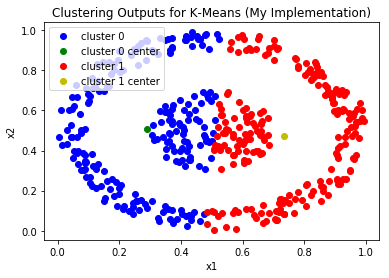
\includegraphics[scale=0.6]{q3c1.png}
	
	Hierarchical Agglomerative Clustering:
	
	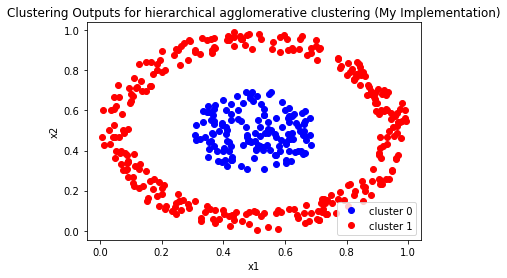
\includegraphics[scale=0.6]{q3c2.png}
	
	From the visualization, we can tell the hierarchical agglomerative clustering algorithm performs better. 
	
	On this specific dataset, possible reasons for the discrepancy are:
	
	\begin{itemize}
		\item K-Means assumes the variance of each X variable is spherical. However, the given data don't satisfy this assumption.
		
		\item The data already form some evident clusters (separated), and the hierarchical agglomerative clustering usually works better in this case.
	\end{itemize}
	
	\item Possible preprocessing on data to make K-Means perform better: move the data to center at $[0, 0]$ (subtract $\bar{x_1}$ from $x_1$, and subtract $\bar{x_2}$ from $x_2$), and turn the data represented by cartesian coordinates into polar coordinates ($[\rho, \theta]$). Then run K-Means on the $\rho$ values of all data. Because points in the same cluster all have similar $\rho$ values. 
	
\end{enumerate}
\end{document}
